\documentclass{article}
\usepackage[spanish]{babel}
	\deactivatetilden
\spanishdecimal{.}
\addto\captionsspanish{\def\tablename{Tabla}}
\addto\captionsspanish{\def\listtablename{\'Indice de tablas}}
\usepackage[numbers,sort&compress]{natbib}
\usepackage[T1]{fontenc}
\usepackage[utf8]{inputenc}
\usepackage{graphicx}
\usepackage{url}
\usepackage{graphicx}
\graphicspath{{Figuras/}}
\usepackage[numbers,sort&compress]{natbib}
\usepackage[clearempty,pagestyles]{titlesec}
\usepackage{anysize}
\usepackage{xcolor, colortbl}
\usepackage{array, multirow, multicol}
\usepackage{enumerate} 

\def\baselinestretch{1.5}
\papersize{27.9cm}{21.5cm} 
\marginsize{2cm}{2cm}{1cm}{1cm}

\title {Interacciones entre partículas}
\author{Julio Garc\'ia}
\pagestyle{empty}

\pagestyle{empty}
\begin{document}
	\renewcommand{\listtablename}{Índice de tablas}
	\renewcommand{\tablename}{Cuadro}
	\maketitle
	
	\section{Introducción}
	En el presente trabajo se busca como objetivo principal el implementar en una interacción de partículas la atracción entre ellas debido a la masa que poseen, dicha implementación parte de una interacción de partículas en la que ya se toma en cuenta la carga que posee cada una de ellas.  
	
	\section{Desarrollo}
	En este trabajo se realiza una extensión al modelo de interacción entre partículas que toma en cuenta la atracción/repulsión debido a la carga que poseen. En esta extensión se toma en cuenta también la atracción que ejerce cada partícula sobre las demás debido a la masa que posee cada una de ellas con respecto a la masa total de las partículas existentes.
	
	\section{Experimentación y resultados}
	En esta sección se describe el ambiente computacional y los resultados obtenidos con la simulación. El código de dicha simulación fue realizado en el lenguaje computacional Python en una computadora personal con procesador 1 Intel Core i7, con memoria RAM de 16GB y hasta 8 núcleos de procesamiento. Dicho código fue incorporado en el repositorio \cite{p_9}.  Se tomó como base el código de Elisa Schaeffer \cite{p9}, en el que se realizaron las variaciones requeridas.\\
	La definición de la atracción entre partículas toma los siguientes supuestos:
	\begin{enumerate}
	\item Hay atracción entre todas las partículas debido a su masa. Esta fuerza nunca hará que las partículas se alejen, siempre se atraen entre ellas.
	\item La fuerza de atracción debido a las masas es proporcional al producto de las masas de las dos partículas en cuestión e inversamente proporcional a la distancia euclidiana entre las partículas (se toma como base la ley de la gravitación, pero sin tomar la constante de gravitación universal para que el efecto sea notorio).
	\item Al momento de graficar ahora el tamaño de la partícula está relacionado con la masa que posee.
	\end{enumerate}
	
	Cabe mencionar que como ahora hay dos fuentes de atracción/repulsión primero se estudia cada una de ellas independientemente, a cada una de ellas se le agregó una constante desde la cual se puede indicar el nivel de afectación debido a esa fuerza correspondiente. Dichas constantes son llamadas alfaCarga y alfaMasa.\\
	
	En primer lugar se realizó experimentación con $alfaCarga = 1$, y $alfaMasa = 0$,  lo cual significa que es el modelo original en el que solamente tiene afectación la carga.
	
	Dicho modelo ya se había comprobado que, si tenía efecto en la posición de las partículas, se presentan un par de imágenes que muestran que las partículas tienden a agruparse al centro de la imagen.
	
	\begin{figure}[h!]
		\centering
		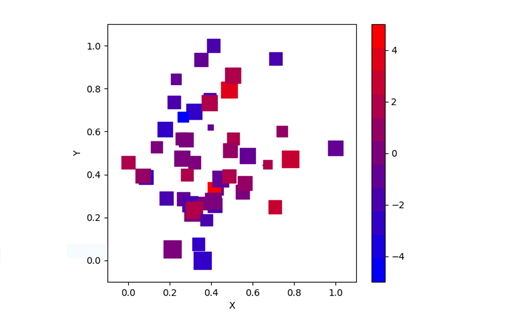
\includegraphics[width=0.7\linewidth]{Figure_1.png}
		\caption{Estado inicial}
		\label{fig:imagen1}
		
		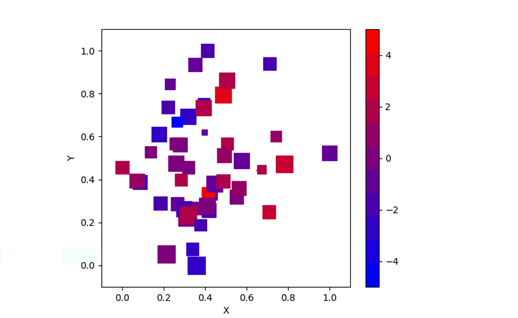
\includegraphics[width=0.7\linewidth]{Figure_2.png}
		\caption{Paso 1}
		\label{fig:imagen2}
		
	\end{figure}
	
		
	\begin{figure}[h!]
		\centering
		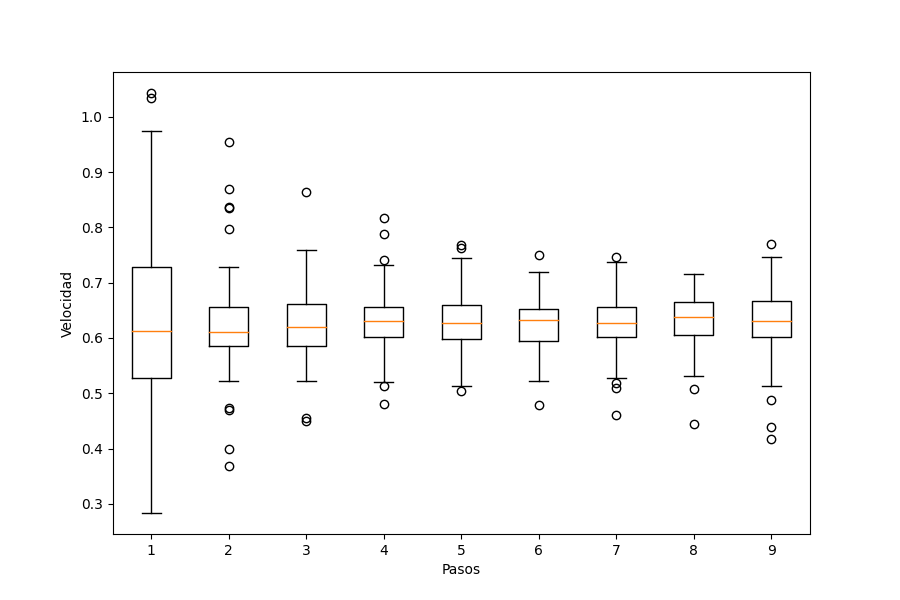
\includegraphics[width=0.8\linewidth]{bx_1.png}
		\caption{Efecto de las masas en la velocidad, primeros $9$ pasos, $alfaCarga=1$, $alfaMasa=0$}
		\label{fig:bx1}
		\end{figure}
	\newpage
	Posteriormente,  se realizó experimentación con $alfaCarga = 0$, y $alfaMasa = 1$,  lo cual significa que es el modelo original en el que solamente tiene afectación la masa, esto con el fin de validar si tiene alguna afectación sobre el comportamiento de las partículas. \\
	
	Como lo muestran las siguientes imágenes este modelo en el que solo se toma en cuenta la atracción debido a la masa de las partículas, también tiene efecto en la posición de las partículas, el comportamiento es muy similar a cuando solo se tomaba en cuenta las fuerzas generadas por las cargas, en este modelo las partículas también tienden a agruparse al centro de la imagen.
	
		\begin{figure}[h!]
		\centering
		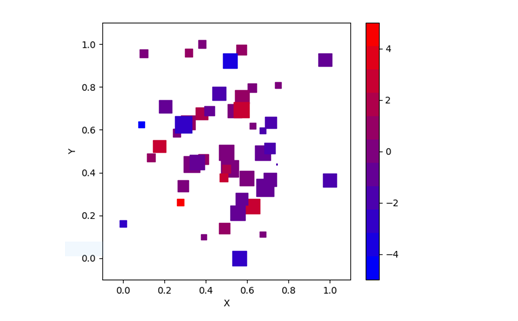
\includegraphics[width=0.7\linewidth]{Figure_3.png}
		\caption{Estado inicial}
		\label{fig:imagen3}
		\end{figure}
		\newpage
		\begin{figure}[h!]
		\centering
		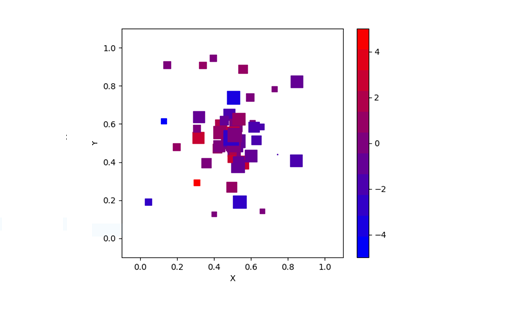
\includegraphics[width=0.8\linewidth]{Figure_4.png}
		\caption{Paso 1}
		\label{fig:imagen4}
		\end{figure}

		\begin{figure}[h!]
		\centering
		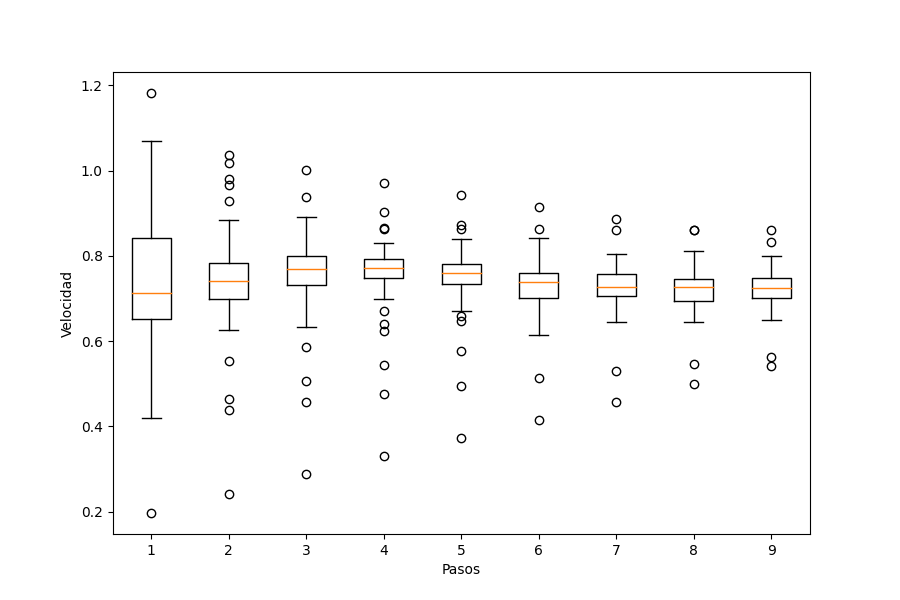
\includegraphics[width=0.8\linewidth]{bx_2.png}
		\caption{Efecto de las masas en la velocidad, primeros $9$ pasos, $alfaCarga=0$, $alfaMasa=1$}
		\label{fig:bx2}
	\end{figure}
    \newpage
	Finalmente se realizó experimentación con $alfaCarga = 1$, y $alfaMasa = 1$,  lo cual significa que tanto la carga como la masa afectan el sistema, esto con el fin de validar la interacción de las dos fuentes de fuerza de atracción/repulsión.
	
			\begin{figure}[h!]
		\centering
		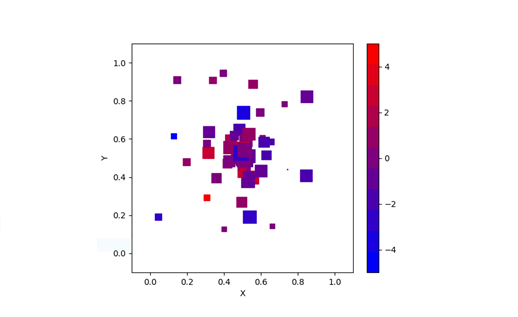
\includegraphics[width=0.8\linewidth]{Figure_5.png}
		\caption{Estado inicial}
		\label{fig:imagen5}
	\end{figure}
	\newpage
			\begin{figure}[h!]
		\centering
		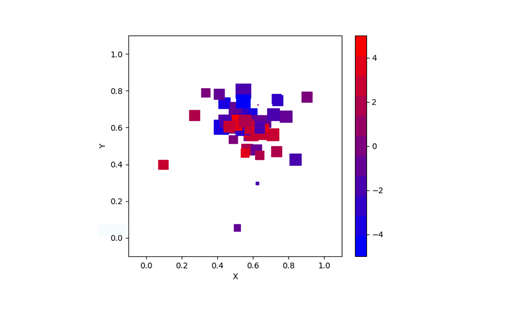
\includegraphics[width=0.9\linewidth]{Figure_6.png}
		\caption{Paso l}
		\label{fig:imagen6}

		\centering
		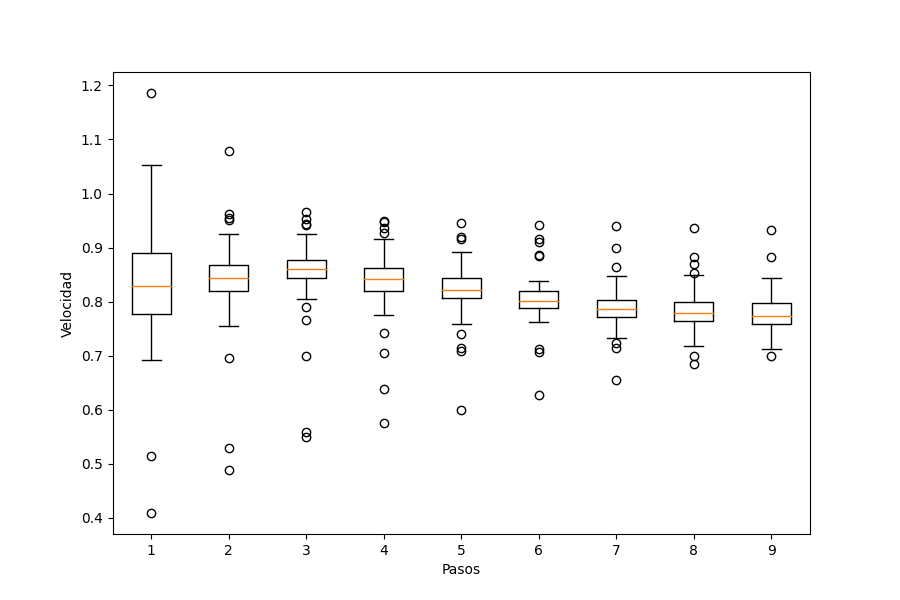
\includegraphics[width=0.8\linewidth]{bx_3.png}
		\caption{Efecto de las masas en la velocidad, primeros $9$ pasos, $alfaCarga=1$, $alfaMasa=1$}
		\label{fig:bx3}
	\end{figure}
	\newpage
	Como lo muestran las siguientes imágenes este modelo en el que se toma en cuenta la atracción debido a la masa de las partículas y también la atracción/repulsión debido a la masa de las mismas, también tiene efecto en la posición de las partículas, el comportamiento es muy similar a cuando solo se tomaba en cuenta las fuerzas generadas por las cargas, en este modelo las partículas también tienden a agruparse al centro de la imagen, sin embargo parecen hacerlo con mucha más rapidez que en los modelos anteriores en los que se estudiaban las fuerzas por separado.
	\section{Conclusiones}
	A continuación, se presentan las conclusiones basados en los resultados y el comportamiento de la posición de las partículas que interactúan entre si:
	\begin{enumerate}
		\item La carga de las partículas si tiene un efecto en el posicionamiento de las mismas conforme pasa el tiempo. 
		\item	La masa de las partículas si tiene un efecto en el posicionamiento de las mismas conforme pasa el tiempo. 
		\item Cuando interactúan la carga y la masa de las partículas, si tienen un efecto en el posicionamiento de las mismas conforme pasa el tiempo y este efecto es mas notorio que cuando se estudian las fuerzas por separado. Este efecto se debe a que la atracción ejercida por las cargas es potenciada por la atracción debida a las masas (las fuerzas generadas a partir de las masas son solamente de atracción).
		
	\end{enumerate}

\bibliography{Biblio}
\bibliographystyle{plainnat}
	
\end{document}